\section{Real-Data Case Studies}\label{sec:realdata}

We now report the first real-data case study using NHANES, with subgrouping by age decade. The analysis uses complete cases for
\{AgeDecade, BMI, Gender, Poverty, DirectChol, Pulse, BPSysAve\}, leaving $n=7116$ observations across $G=8$ groups
($0$--$9$: 186, $10$--$19$: 1080, $20$--$29$: 1126, $30$--$39$: 1138, $40$--$49$: 1217, $50$--$59$: 1116, $60$--$69$: 782, $70+$: 471).

The pooled model is
\[
\mathrm{BMI} \sim \mathrm{Gender} + \mathrm{Poverty} + \mathrm{DirectChol} + \mathrm{Pulse} + \mathrm{BPSysAve},
\]
and we fit the same formula separately within each age decade. We then compute sign stability, standardized drift, context-normalized drift, and predictor-wise objective components.

The aggregate stability summary indicates meaningful subgroup heterogeneity: mean sign stability is $0.814$, mean standardized drift is $16.203$, mean context-normalized drift is $11.339$, and the objective score is $16.389$.

Predictor-level metrics show that BPSysAve is the least stable term in this specification. Its sign stability rate is $0.571$, standardized drift is $32.070$, and context-normalized drift is $17.641$. By contrast, Gendermale and DirectChol have perfect sign stability (SSR $=1.0$), although DirectChol still shows nontrivial magnitude drift.

To visualize coefficient heterogeneity, we generated pooled and subgroup coefficient tables and fitted-curve plots, and added a dedicated BPSysAve coefficient plot with 95\% confidence intervals by age decade. The BPSysAve plot shows a clear decline across age, with sign reversal in the oldest decades.

\begin{figure}[htbp]
\centering
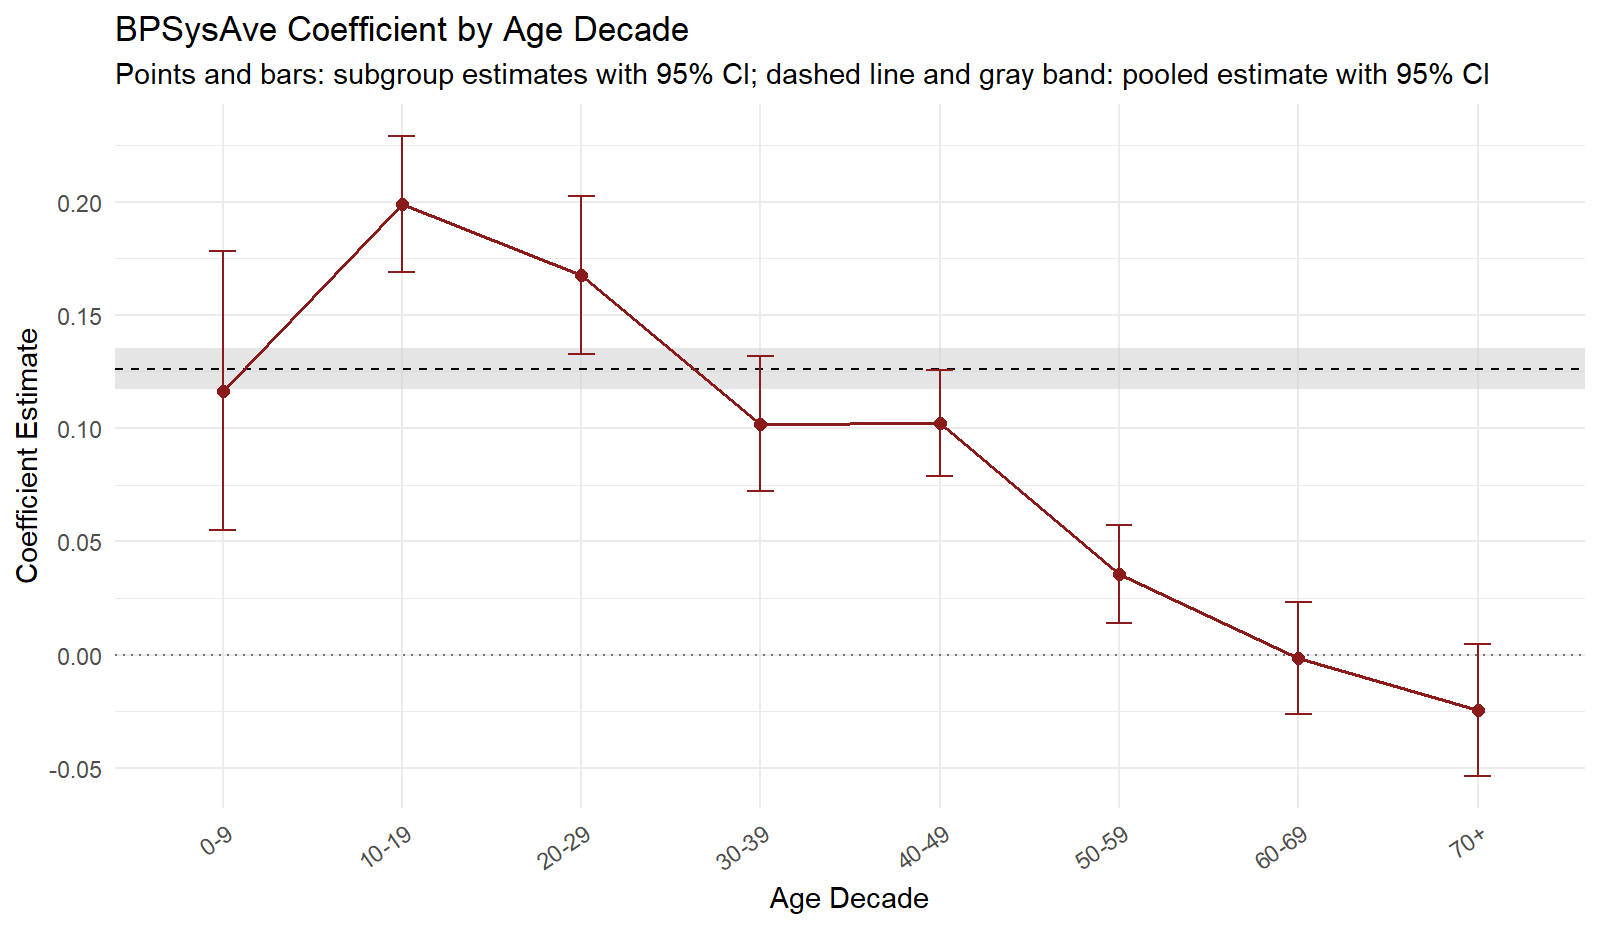
\includegraphics[width=0.82\textwidth]{../results/nhanes_age_decade/bpsys_coef_by_age_decade_ci.png}
\caption{Estimated BPSysAve coefficient by age decade with 95\% confidence intervals. The dashed horizontal line and shaded band show the pooled estimate and its 95\% interval.}
\label{fig:nhanes-bpsys-ci}
\end{figure}

Because the youngest decade has a smaller sample ($n=186$), we ran a size-sensitivity check. Excluding $0$--$9$ reduces several drift values, but does not remove instability for BPSysAve (drift falls from $32.070$ to $28.696$, SSR changes from $0.571$ to $0.524$). Among similarly sized middle-age groups ($10$--$19$ through $50$--$59$), BPSysAve sign agreement is high, while older decades still drive directional mismatch. This pattern supports a regime-change interpretation rather than a pure small-sample artifact.

We also compared pooled versus age-specific predictive accuracy within each decade. Group-specific models improved RMSE and $R^2$ in every decade. The largest pooled failure occurred in $0$--$9$ (pooled $R^2=-3.485$ vs subgroup $R^2=0.241$), while notable gains remained in older groups (for $70+$: pooled $R^2=-0.086$ vs subgroup $R^2=0.130$). These results are consistent with coefficient instability and indicate that one pooled linear rule is not uniformly accurate across age strata.